\documentclass[12pt]{article}
\usepackage[margin=1.5in,dvips]{geometry}
\usepackage{fontspec}
\setmainfont[Ligatures=TeX]{Cambria}
%\usefonttheme{serif}
%\usefonttheme{professionalfonts}
\usepackage{breakurl}
\usepackage{color}
%\usepackage{booktabs} % For formal tables
\usepackage{listings}
\usepackage{amsmath}
\usepackage{amssymb}
\usepackage[mathscr]{euscript}
\usepackage{verbatim}
\usepackage[pdflang={en-US},pdftex]{hyperref}
\usepackage{url}
\usepackage{graphicx}

\renewcommand{\refname}{\normalsize REFERENCES}
\renewcommand\abstractname{\textsc{summary}}

\title{\normalsize \bfseries
PARAREAL ALGORITHM IMPLEMENTATION AND SIMULATION IN JULIA}

\author{\normalsize{Tyler M. Masthay$^{\dagger}$ and Saverio Perugini$^{\ddagger}$}\\
\scriptsize{$^{\dagger}$Institute for Computational and Engineering Sciences, University of Texas Austin, tyler@ices.utexas.edu}\\
\scriptsize{$^{\ddagger}$Department of Computer Science, University of Dayton,
Ohio\ \ 45469--2160, saverio@udayton.edu}}

\begin{document}
\sloppy
\date{\normalsize{August 16, 2018}}

\maketitle
\thispagestyle{empty}
\pagestyle{empty}

\begin{abstract} We present an implementation of the parareal algorithm—an
integration technique to solve differential equations in parallel---first
proposed in 2001 by Lions, Maday, and Turinici~\cite{Lions:2001}---in the Julia
programming language~\cite{Julia:2014} for a fully general, first-order,
initial-value problem.  We also provide a graphical simulation of the parareal
algorithm intended to be used in a numerical analysis course to both introduce
the parareal algorithm to students and aid them in an investigation of the
types of curves for which the parareal algorithm might be practical.  Our
implementation of the parareal algorithm accepts both coarse and fine
integrators as functional arguments.  We provide implementations of Euler’s
method and another Runge-Kutta integration technique as the integrators.  The
final two functions in the source code file \texttt{parareal.jl} are functions
implementing Euler’s method and another Runge-Kutta integration technique that
can be used as examples to be passed as first-class functions as coarse or fine
integration techniques to the \texttt{parareal} or \texttt{simulate} functions.
A Git repository of both the implementation and graphical simulation is
available in GitHub at
\url{https://github.com/sperugin/Parareal-Implementation-and-Simulation-in-Julia.git}.
All of the graphical plots are generated with the Julia Plots package available
at \url{https://juliaplots.github.io/}.  A video describing this application of
Julia is available on YouTube at
\url{https://www.youtube.com/watch?v=MtgbeLO6ZM4}.  The purpose of this
software is pedagogical: as a simulation to introduce students to the parareal
algorithm and the concept of concurrency, and as a tool for (graphically)
investigating the performance of the algorithm.  \end{abstract}

\paragraph{Keywords:}
Concurrent programming,
\textit{Euler's method},
Julia,
\textit{Runge-Kutta} methods,
parareal algorithm,
ordinary differential equations.

\section*{\normalsize THE PARAREAL ALGORITHM}

\begin{figure}
\centering
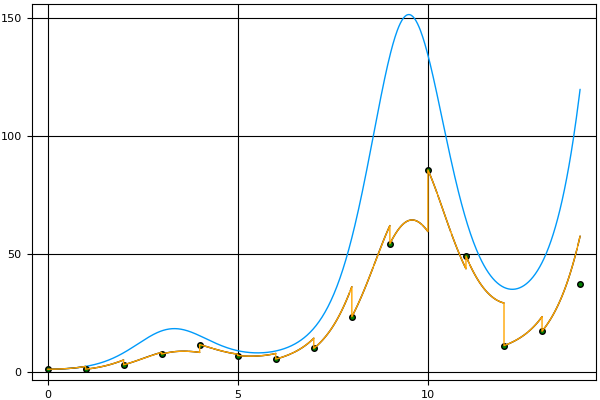
\includegraphics[scale=0.55]{error.png}
\caption{Right endpoint error.}
\label{errorIllustration}
\end{figure}

The parareal algorithm is designed to perform parallel-in-time integration for
a first-order initial-value problem.  The algorithm involves two integration
techniques, often known as the `coarse' integrator and the `fine'
integrator. For the algorithm to be effective, the coarse integrator must be of
substantially lower computational cost than the fine integrator. The reason
will become apparent later in this section.   Consider the differential
equation $\eqref{ode}$ given by

\begin{equation}\label{ode}
y'(t) = f(t,y(t)) \quad t \in [a,b]
\end{equation}

\noindent
with its associated initial-value problem $\eqref{ivp}$
\begin{equation}\label{ivp}
y(t^{*}) = y^{*} \quad t^{*} \in [a,b]\mathrm{.}
\end{equation}

\noindent For simplicity, let us assume $t^{*} = a$, so that the solution only
extends rightward.  To obtain an approximate solution to equation~$\eqref{ode}$
satisfying the initial condition~$\eqref{ivp}$, we partition our domain into
$[t_0=a,...,t_N=b]$ with uniform step size $\Delta$.
We now precisely define an `integrator' as a function from $(0,\infty) \times \mathbb{R}^{2} \times \mathscr{R}$ to $\mathbb{R}$ where $\mathscr{R}$ is the set of all Riemann integrable functions. For example, the integrator $I$ given by 
\begin{equation*}
I(\delta,x_0,y_0,g) = y_0 + g(x_0,y_0)\delta
\end{equation*}

\noindent
is the integrator corresponding to Euler's method with step size $\delta$.
Let $\mathscr{C}$ and $\mathscr{F}$ be the coarse and fine integrators,
respectively. Define
\begin{align*}
   y_{0,1} &= y(t_0) = y^{*} \\
    y_{n+1,1} &= y(t_{n+1}) = \mathscr{C}(\Delta,t_n,y_{n,1},f)\mathrm{.}
\end{align*}

\noindent
Since $y_{n+1,1}$ depends on $y_{n,1}$, this algorithm is inherently
sequential. Partition $[t_n,t_{n+1}]$ into
$\{t_{n}^{0}=t_n,...,t_{n}^{m},...t_{n}^{M}=t_{n+1}\}$ with uniform step size $\delta < \Delta$. Define 
\begin{align*}\label{parallelDiscrete}
   z_{n,1}^{0} &= y(t_{n}^{0}) = y_{n,1} \\
    z_{n,1}^{m+1} &= y(t_{n}^{m+1}) = \mathscr{F}(\delta,t_{n}^{m},z_{n,1}^{m},f)\mathrm{.}
\end{align*}

\noindent
This yields an approximate solution $\{z_{n,1}^{0},...,z_{n,1}^{M}\}$ to
$\eqref{ode}$ over $[t_n,t_{n+1}]$ with initial conditions
\begin{align*}
   y(t_{n}) = y_{n,1}\mathrm{.}
\end{align*}

\noindent Since $z_{n_1,1}^{m_1}$ does not depend on $z_{n_2,1}^{m_2}$ for $n_1
\neq n_2$, we can compute these approximations in parallel. After the last
subproblem is solved, we simply combine the solutions on each subdomain to
obtain a solution over the whole interval. However, our values $\{
y_{1,1},...,y_{n,1} \}$ are relatively inaccurate. The vertical spikes in the
orange graph separating the coarse and fine predictions in
Figure~\ref{errorIllustration} illustrate this error.  However, $z_{n-1,1}^{M}$
is a better approximation for $\phi(t_n)$
 where $\phi$
is the exact solution to the differential equation.
We use this to obtain a 
better set of points $\{y_{n,2}\}$ for the coarse approximation. We do this by first defining $w_{n,1} = y_{n,1}$ and then defining
\begin{align*}
w_{1,2} &= y_{1,1} = y_{1,2} = y^{*} \\
w_{n,2} &= \mathscr{C}(\Delta,t_{n-1},y_{n-1,2},f)\\
y_{n,2} &= (w_{n,2}-w_{n,1}) + z_{n-1,1}^{M}\mathrm{.}
\end{align*}
Thus, $w_{n+1,2}$ serves as a new prediction given a more accurate previous prediction from $y_{n,2}$ since $z_{n-1,1}^{M}$ has now been taken into account in calculating $y_{n,2}$. In general, we continue evaluating so that for
$k > 1$, we have
\begin{align*}
w_{1,k} &= y_{1,k} = y^{*} \\
w_{n,k} &= \mathscr{C}(\Delta,t_{n-1},y_{n-1,k-1},f)\\
y_{n,k} &= (w_{n,k}-w_{n,k-1}) + z_{n-1,k-1}^{M}\mathrm{.}
\end{align*}

\noindent Note that since $y_{n,k}$ is dependent on $w_{n,k}$, this step must
be done sequentially. As $k$ increases, $w_{n,k} - w_{n,k-1} \to 0$, which
means that $y_{n,k}$ converges to the value that the fine integrator would
predict if fine integration were simply done sequentially. Thus, each $k$
denotes fine integration over the whole interval. This means that the total 
computation performed is much greater than if fine integration were performed
sequentially.  However, the time efficiency of each iteration has the potential
to be improved through concurrency. Since fine integration is more
computationally intensive, this improvement in the run-time efficiency may
compensate for the cumulative computation performed.

Let $K$ be the total number of iterations necessary to achieve a desired
accuracy of solution and $P$ be the number of subintervals into which we divide 
according to the coarse integrator. If $K=1$, then we achieve perfect parallel
efficiency. If $K = P$, then we likely slowed the computation down. The
parareal algorithm is guaranteed to converge to the solution given by the
sequential fine integrator within $P$ iterations. For a more complete treatment
of this convergence analysis, we refer the reader to~\cite{Gander:2007}. For fully
general pseudocode, we refer the reader to~\cite{Aubanel:2011,Nielsen:2012}. 

\section*{\normalsize PARAREAL ALGORITHM IMPLEMENTATION IN JULIA}

The \texttt{@async} macro within the loop causes the program to
evaluate the first expression to its right as a concurrent task (i.e., the
\texttt{for} loop assigning values to \texttt{sub}).  The \texttt{@sync} macro
causes the main program thread to wait until all tasks (spawned in the the
first expression to its right with an \texttt{@async} or \texttt{@parallel}
macro) complete.  Once all concurrent tasks are complete, execution of the
program proceeds sequentially. Given the semantics of these macros, the program
correctly perform concurrent integration.  The sequential and parallel versions
of this implementation have no significant differences in run-time efficiency.
However, if a \texttt{sleep} statement is placed in the argument of
\texttt{fineIntegrator}, the parallel version runs much faster.  This
demonstrates that use of those two macros leads to concurrent program
execution.

\section*{\normalsize GRAPHICAL ALGORITHM SIMULATION}

\begin{figure}
\resizebox{\textwidth}{!}{
\begin{tabular}{cc}
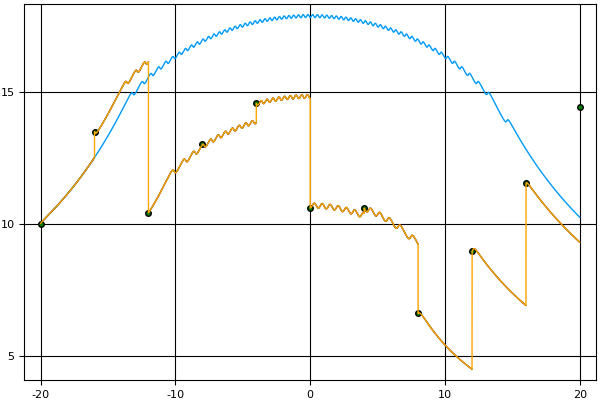
\includegraphics[scale=1.0]{sin1.png} &
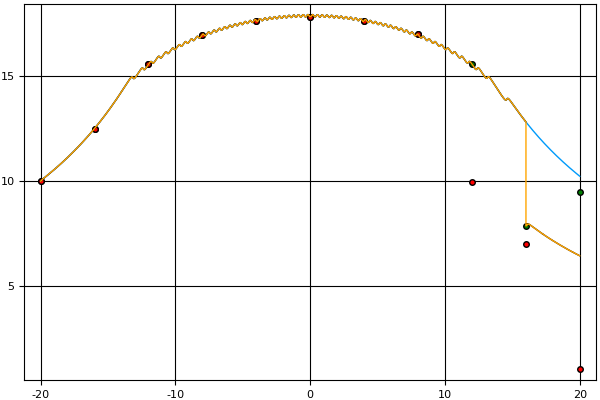
\includegraphics[scale=1.0]{sin2.png}
\end{tabular}}
\caption{Slow parareal
example. (left) Solution after first iteration with Euler's method. (right)
Solution after ninth iteration with Euler's method.}
\label{sinPara}
\end{figure}

The function \texttt{simulate} creates a graphical simulator of the parareal
algorithm and can be used to introduce the parareal algorithm to students in a
numerical analysis course.  The first line gets the sequential solution from
the fine integrator (the `ideal' solution) and the second line gets the history
of the computations that took place during the parareal execution. The main
loop over the variable $k$ then displays the inner workings of the algorithm.
The ideal solution is plotted, with a scatter plot of the points obtained from
the coarse integrator. To simulate the parallel nature of the algorithm, random
progress is made on randomly selected subdomains. Thus, the plot dynamically
makes partial progress on different subdomains until all subdomains are
finished with the fine integration. After this, the plots are connected into
the current iteration's approximation. During the next iteration, the previous
guesses from the coarse integrator are displayed in red and the new guesses
from the coarse integrator are displayed in green. As $k$ increases, these
guesses converge to the ideal solution.

In addition to the use of this function for pedagogical purposes, it can be
used to investigate the types of curves for which the parareal algorithm might
be practical.  For instance, consider the differential equation

\begin{equation*} y'(x) = sin(xy), \quad x \in [-20,20] \end{equation*}

\noindent with $y(-20) = 10$, $\Delta = 4$ (10 points), and $\delta = 0.008$
(500 points).  Figure~\ref{sinPara} shows the first and ninth iterations.  The
ninth iteration's large error on the right end of the interval shows that this
is an example where parareal convergence is slow. This is as inefficient as
possible, needing as many iterations as subdomains in order for the solution to
converge.  However, the simulation also shows that if $f(x,y) = sin(x)e^x$,
then the solution converges after just one iteration.  These two examples show
that the algorithm's efficiency can be highly dependent on the integrand. 

\bibliographystyle{plain}
\bibliography{parareal} 

\end{document}
